\subsection{Introduction}
\begin{frame}{Contexte}
\begin{block}{Expériences numériques comme aide à la conception / décision}
 \begin{itemize}
  \item Réponse du code de calcul = performance ou coût
  \item Recherche des paramètres optimaux :
  $$x^* = \arg \min cout(x) \text{ ou } \arg \max {perf(x)}$$
  \item L'optimisation nécessite beaucoup d'appels au code
  \item Métamodèle : solution naturelle
 \end{itemize}
\end{block}

\begin{exampleblock}{Lien avec la problématique précédente}
Le métamodèle doit être précis seulement dans les régions importantes (proche de l'extremum)
$\Rightarrow$ répartition des expériences ``ciblée''
\end{exampleblock}

\begin{alertblock}{Démarche nécessairement séquentielle}
Il faut faire des expériences pour connaître les régions cibles !
\end{alertblock}
\end{frame}
%-----------------------------------------------------
\begin{frame}
  \frametitle{Planification d'expériences et optimisation globale}
  \begin{block}{Optimisation locale}
Amélioration depuis un point initial
  \end{block}

  \begin{block}{Optimisation globale : le \textbf{compromis exploration / intensification}}
  \begin{itemize}
   \item Exploration : recherche partout dans l'espace pour ne pas rater la zone optimale 
   \item Intensification : une fois une zone identifiée : on recherche le minimum local
  \end{itemize}
  \end{block}
  
\begin{exampleblock}{Dans un contexte de planification d'expériences}
  \begin{itemize}
   \item Exploration : remplissage d'espace
   \item Intensification : ``ciblage''
  \end{itemize}
\end{exampleblock}
  
\end{frame}
%-----------------------------------------------------
\begin{frame}
  \frametitle{Introduction à l'optimisation globale : l'algorithme DIRECT}
  Garanti sans métamodèle !
  \begin{block}{DIRECT : DIviding RECTangles}
  \begin{itemize}
   \item Découpage de l'espace en (hyper)rectangles
   \item Un échantillon au centre de chaque rectangle
   \item On divise les rectangles les plus ``intéressants'' :
   \begin{itemize}
     \item soit les plus grands (exploration)
     \item soit ceux qui ont une valeur au centre basse (intensification)
   \end{itemize}
   \item Pour diviser : ajout de 2 points, division en 3
  \end{itemize}
  \end{block}
  \scriptsize{
 \begin{thebibliography}{7}
\beamertemplatearticlebibitems
%\beamertemplatebookbibitems
     \bibitem{direct}
     D.~Jones, C.~Perttunen, B.~Stuckman (1993)
         \newblock Lipschitzian optimization without the Lipschitz constant
         \newblock Journal of Optimization Theory and Applications 79(1), 157-181
 \end{thebibliography}
}
\normalsize
%   \begin{block}{Compromis exploration / intensification}
% Pour (presque) \textbf{chaque} taille de rectangle, on divise celui qui a la meilleure valeur observée
%   \end{block}
%   
\end{frame}
%-----------------------------------------------------
\begin{frame}
\frametitle{Exemple en dimension 2}
%   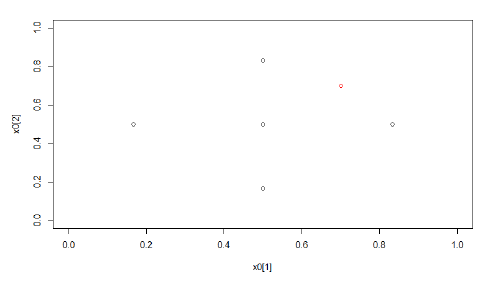
\includegraphics[width=.45\paperwidth]{fig/direct1.png}
%   \\
\begin{itemize}
 \item Départ : 3 points équirépartis dans une direction aléatoire
 \item On divise le rectangle ayant la meilleure observations
\end{itemize}

  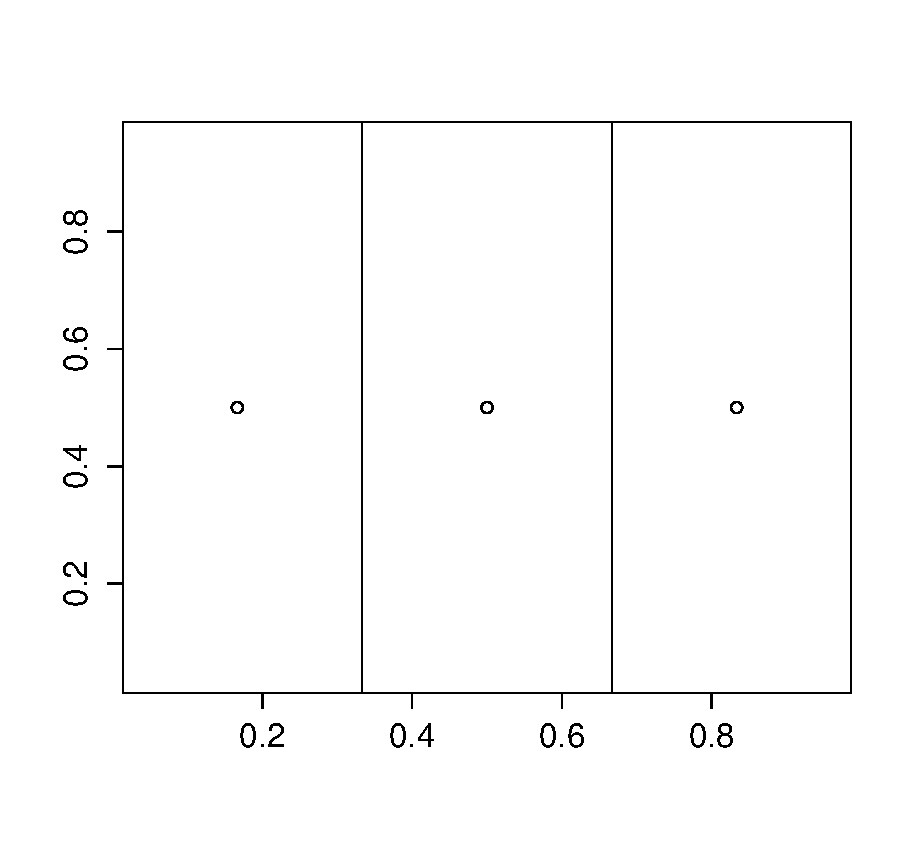
\includegraphics[width=.45\textwidth]{fig/direct1.pdf} \hspace{5mm}
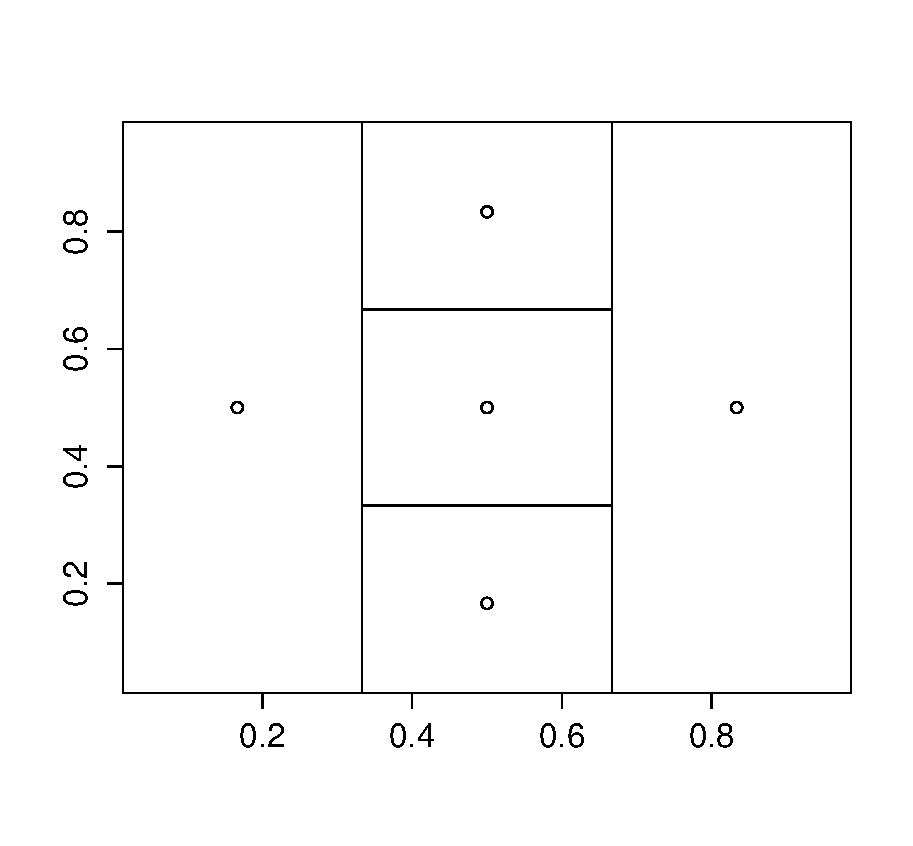
\includegraphics[width=.45\textwidth]{fig/direct1bis.pdf}
  \end{frame}

%-----------------------------------------------------
\begin{frame}
\frametitle{Exemple en dimension 2}
%   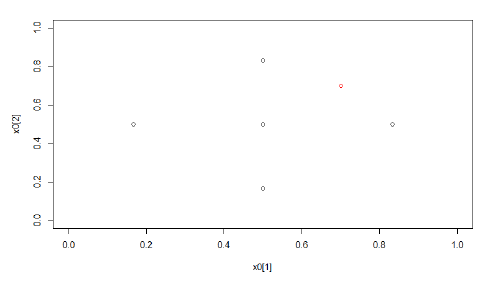
\includegraphics[width=.45\paperwidth]{fig/direct1.png}
%   \\
  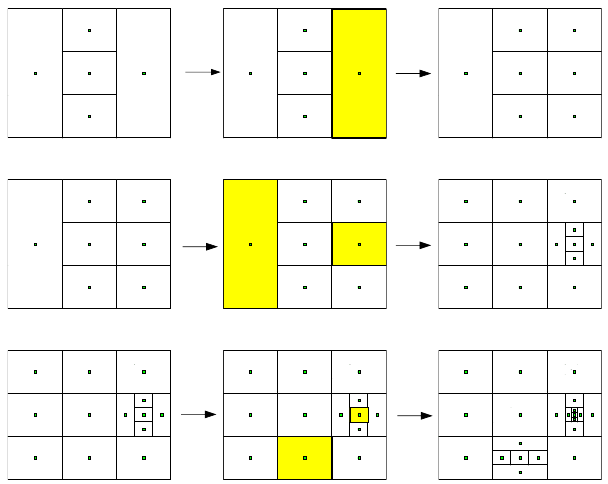
\includegraphics[width=.9\textwidth]{fig/direct2.png}
\end{frame}

%-----------------------------------------------------
\begin{frame}
\frametitle{Après 191 évaluations}
\begin{itemize}
 \item Echantillonnage intense dans la zone de l'optimum
 \item Bonne exploration 
\end{itemize}



\begin{columns}
 \begin{column}{80mm}
 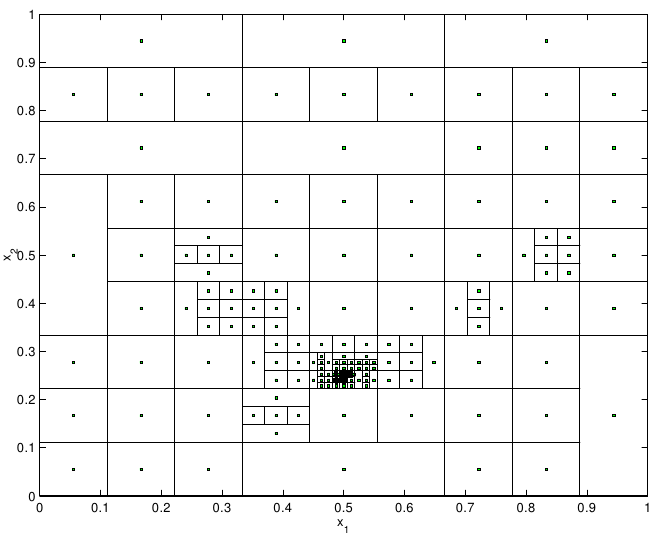
\includegraphics[width=\textwidth]{fig/direct3.png}  
 \end{column}
 \begin{column}{40mm}
   \scriptsize{Source figures :
 \begin{thebibliography}{1}
\beamertemplatearticlebibitems
     \bibitem{fin}
     D. E. Finkel
         \newblock DIRECT Optimization Algorithm User Guide (2003)
 \end{thebibliography}}
 \end{column}
\end{columns}
\end{frame}
%-----------------------------------------------------
\begin{frame}
\frametitle{Intêret et limites}
\begin{itemize}
 \item[$+$] Exploration de tout l'espace de recherche
 \item[$+$] Stratégie robuste
 \item[$-$] Limité aux petites dimensions
 \item[$-$] Exploitation limitée de l'information
\end{itemize}
\vspace{5mm}
$\Rightarrow$ même principe général, avec un métamodèle ?
\end{frame}
%-----------------------------------------------------
% \subsection{Optimisation et métamodèles}
%-----------------------------------------------------
\begin{frame}
\frametitle{Optimisation et métamodèle : ce qu'on est tenté de faire...}
\begin{columns}[l]
 \begin{column}{.51\textwidth}
  
\begin{block}{``Le métamodèle donne l'optimum''}
 \begin{itemize}
  \item On cherche le minimum $x^*$ sur le métamodèle
  \item On évalue le vrai $y(x^*)$ sur le simulateur
 \end{itemize}
$\Rightarrow$ C'est fini !
\end{block}

\begin{block}{Répartition de l'effort}
 \begin{itemize}
  \item Plan initial : 49 expériences
  \item 98\% exploration, 2\% exploitation
 \end{itemize}
\end{block}
 \end{column}
 \begin{column}{.49\textwidth}
  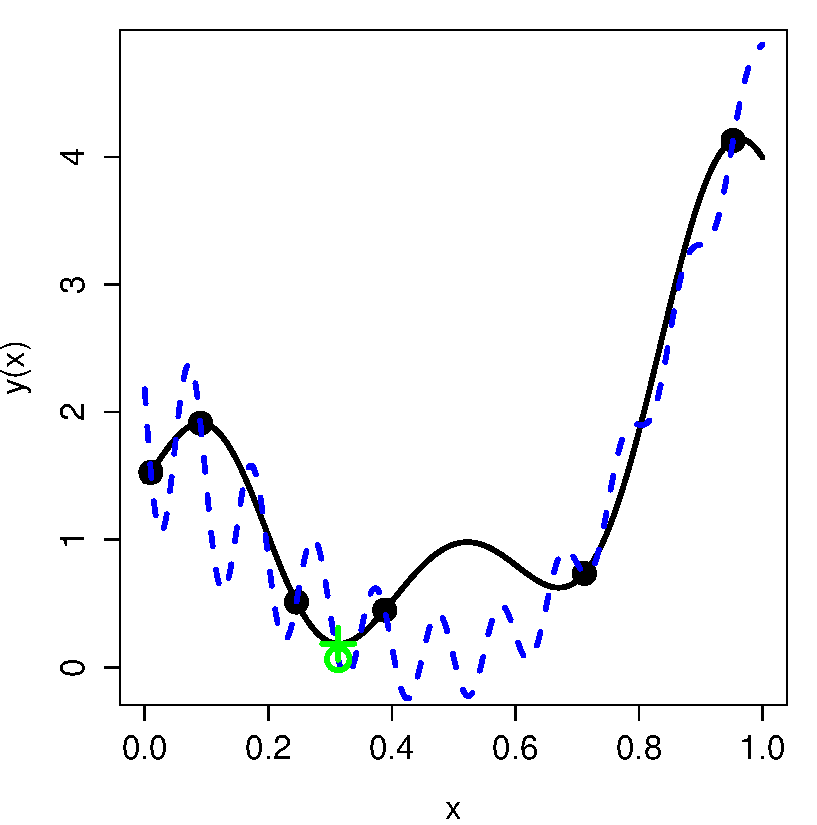
\includegraphics[width=\textwidth]{fig/exoptim1.pdf}
 \end{column}
\end{columns}
\vspace{1mm}
\centering
\textcolor{red}{Que faire si $x^*$ n'est pas bon ?}
\end{frame}

%-----------------------------------------------------
\begin{frame}
\frametitle{Optimisation et métamodèle : ce qu'il faut faire}
\begin{block}{Si le budget est fixe}
 \begin{itemize}
  \item On divise le budget en 2
  \item Budget 1 : plan initial (LHS)
  \item Budget 2 : optimisation
 \end{itemize}
\end{block}

\begin{block}{Utilisation \textbf{séquentielle} du métamodèle}
 \begin{itemize}
  \item Métamodèle initial : \textit{a priori} peu précis
  \item Le métamodèle sert à \textbf{choisir} pour les nouvelles observations
  \item A chaque nouvelle observation : amélioration du métamodèle
 \end{itemize}
\end{block}
\end{frame}

% %-----------------------------------------------------
% \begin{frame}
% \frametitle{Schéma général : métamodèle = guide}
% 
%    \begin{tikzpicture}[scale=1]
%    \draw(6,2) rectangle (11,3);
%    \draw(8.5,2.5) node{PX initial};
%    
%    \draw[<-,thick] (5,2.5)--(6,2.5);
%    
%    \draw(0,2) rectangle (5,3);
%    \draw(2.5,2.5) node{Simulations};
%    
%    \draw[<-,thick] (2.5,1)--(2.5,2);
%    
%    \draw(0,0) rectangle (5,1);
%    \draw(2.5,.5) node{Construction du métamodèle};
%  \draw[<-,thick] (2.5,-1)--(2.5,0);
%     \draw(0,-2) rectangle (5,-1);
%    \draw(2.5,-1.5) node{Choix de la nouvelle xp};
%  \draw[<-,thick] (2.5,-3)--(2.5,-2);
%      \draw(0,-4) rectangle (5,-3);
%    \draw(2.5,-3.5) node{Simulation};
%   
%   \draw[->,thick] (5,-3.5)--(6,-3.5);
%   
%    \draw(6,-4) rectangle (11.5,-3);
%    \draw(8.75,-3.5) node{Enrichissement du métamodèle};
%   \draw[-,thick] (8.75,-3)--(8.75,-1.5);
%   \draw[<-,thick] (5,-1.5)--(8.75,-1.5);
%  \end{tikzpicture}
% \end{frame}

%-----------------------------------------------------
\subsection{Optimisation basée sur les modèles polynomiaux}
%-----------------------------------------------------
\begin{frame}
\frametitle{Optimisation basée sur les modèles polynomiaux}
\begin{block}{Principe}
 \begin{itemize}
  \item On construit une surface de réponse $y = \beta_0 + \beta_1 x + \beta_2 x^2$
  \item On cherche le point qui minimise la surface de réponse
  \item On ajoute ce point
  \item On met à jour la surface de réponse
  \item On recommence...
 \end{itemize}
\end{block}

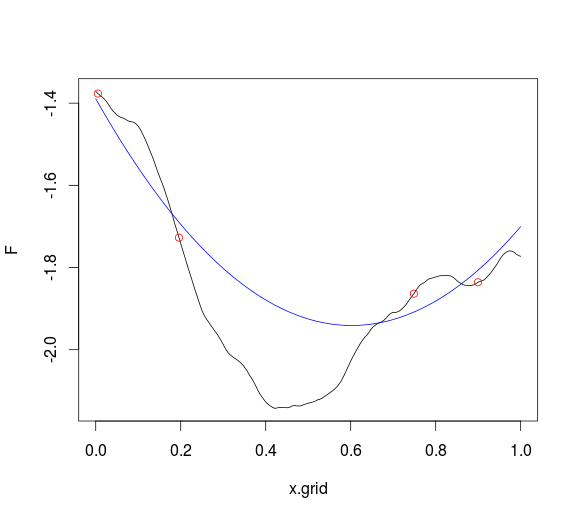
\includegraphics[trim = 10mm 20mm 10mm 10mm, clip, width=.37\paperwidth]{fig/prs1.png}
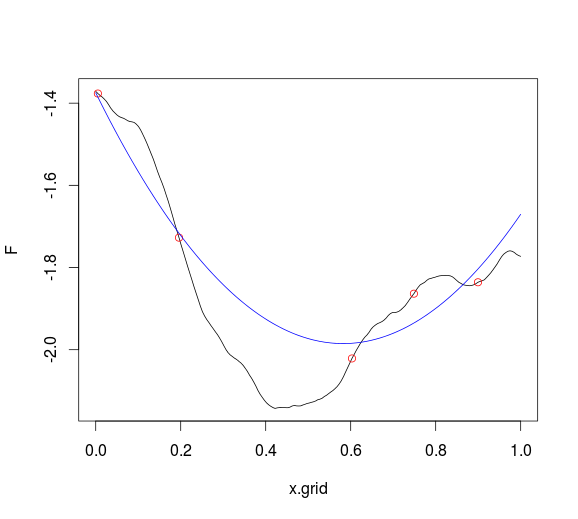
\includegraphics[trim = 10mm 20mm 10mm 10mm, clip, width=.37\paperwidth]{fig/prs2.png}
\end{frame}

%-----------------------------------------------------
%-----------------------------------------------------
\begin{frame}
\frametitle{Itérations 3 à 7}
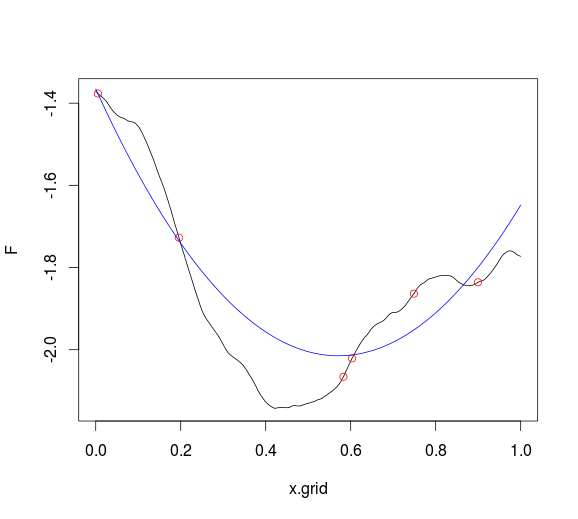
\includegraphics[trim = 10mm 20mm 10mm 10mm, clip, width=.3\paperwidth]{fig/prs3.png}
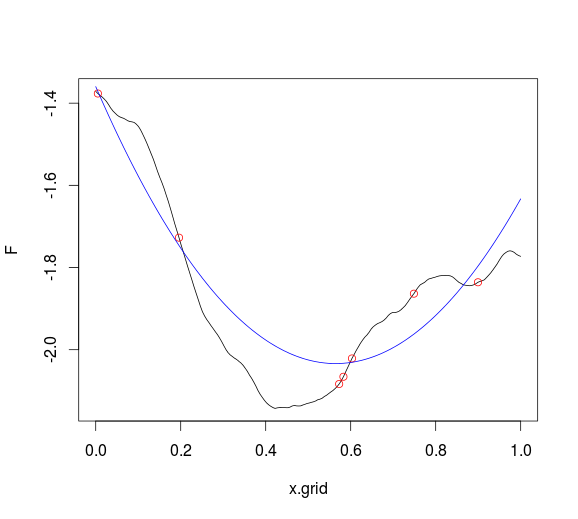
\includegraphics[trim = 10mm 20mm 10mm 10mm, clip, width=.3\paperwidth]{fig/prs4.png}
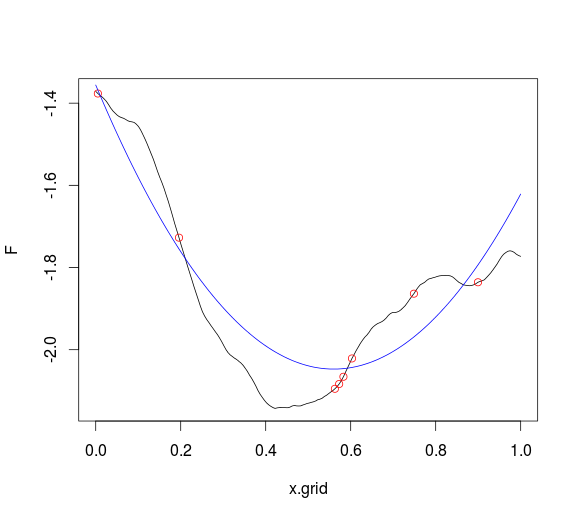
\includegraphics[trim = 10mm 20mm 10mm 10mm, clip, width=.3\paperwidth]{fig/prs5.png}
\\
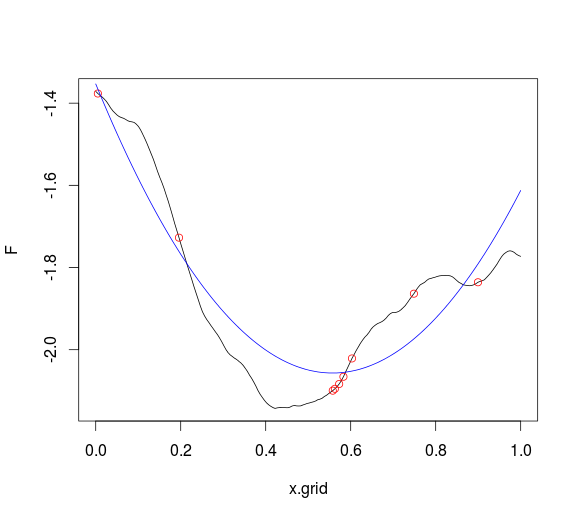
\includegraphics[trim = 10mm 20mm 10mm 10mm, clip, width=.3\paperwidth]{fig/prs6.png}
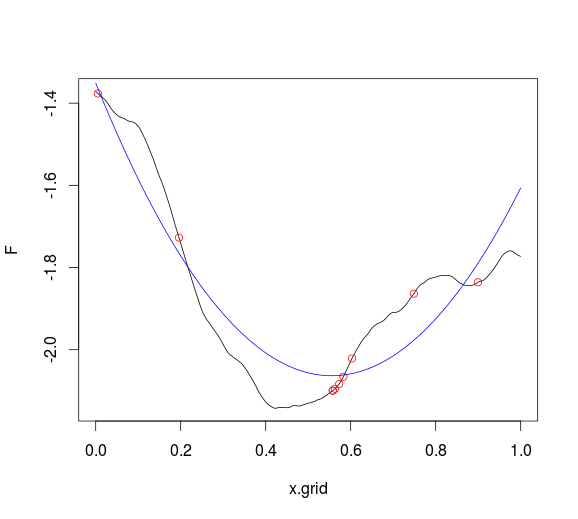
\includegraphics[trim = 10mm 20mm 10mm 10mm, clip, width=.3\paperwidth]{fig/prs7.png}
\end{frame}
%-----------------------------------------------------
\begin{frame}
\frametitle{Optimisation basée sur les modèles polynomiaux}
\begin{block}{Problème : modèle ``rigide''}
Le modèle ne s'ajuste pas aux données : 
$ Y = \mathbf{X} \beta + \epsilon $

Pas de convergence vers un modèle précis, même localement
\end{block}

\begin{exampleblock}{Solutions}
\begin{enumerate}
 \item Augmenter le dégré du polynôme \\
 \textcolor{red}{$\Rightarrow$ risque de surapprentissage \& d'instabilité !}
 \item Supprimer des points \\
 $\Rightarrow$ méthode \textbf{de région de confiance}
\end{enumerate}
\end{exampleblock}
\end{frame}

%-----------------------------------------------------
\begin{frame}
\frametitle{Régions de confiance : principe}
\begin{block}{Modèle quadratique ``creux''}
\begin{itemize}
 \item Valide à l'intérieur d'une région de confiance (petite)
 \item Construit uniquement avec les points à l'intérieur de la région
 \item Selon les valeurs des simulations, on modifie la taille de la région
\end{itemize}
\end{block}

\begin{block}{Gestion de la région de confiance}
A chaque itération :
\begin{itemize}
 \item $\hat y (x^*)$ bon $\Rightarrow$ confiance dans le modèle : on augmente la taille
 \item $\hat y (x^*)$ mauvais $\Rightarrow$ modèle peu fiable : on diminue la taille
\end{itemize}
\end{block}
+ beaucoup de règles pour sélectionner les points et enrichir le plan d'expériences
\end{frame}
%-----------------------------------------------------
\begin{frame}
\frametitle{Illustration (source : F. Vanden Berghen)}
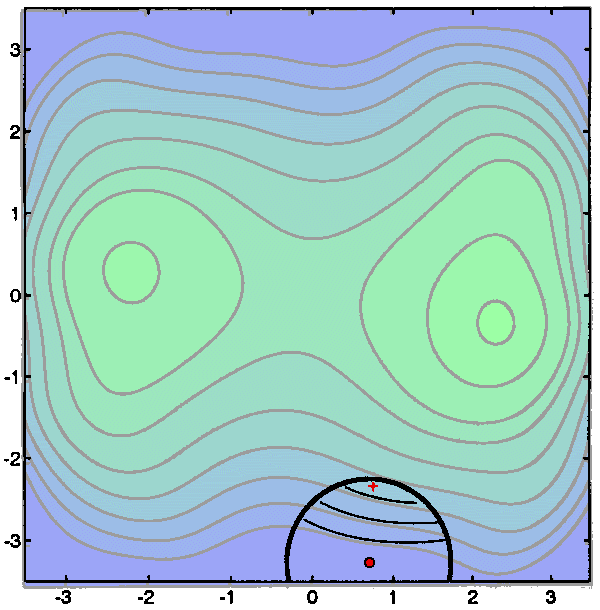
\includegraphics[width=.5\textwidth]{trm/Image2.png}
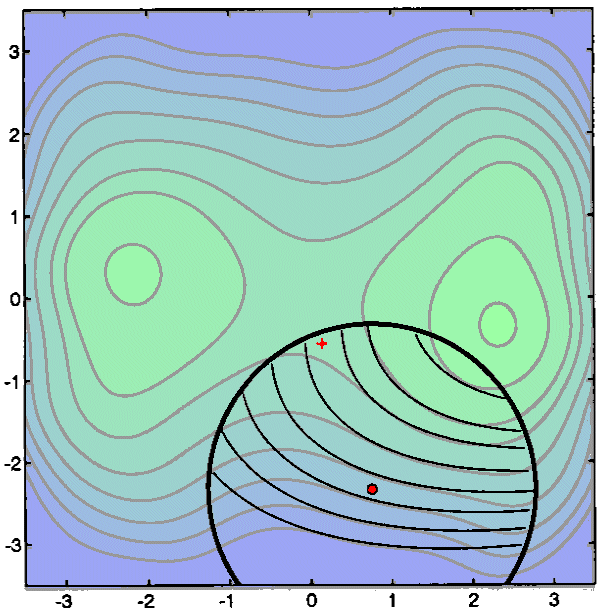
\includegraphics[width=.5\textwidth]{trm/Image3.png}
\end{frame}
%-----------------------------------------------------
\begin{frame}[noframenumbering]
\frametitle{Illustration (source : F. Vanden Berghen)}
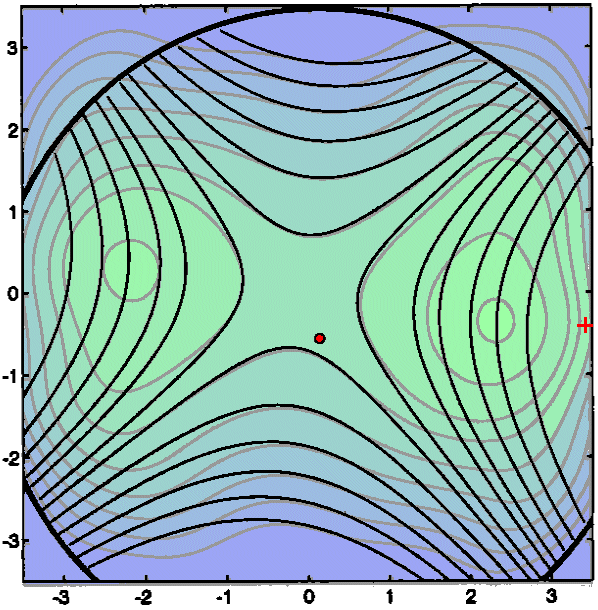
\includegraphics[width=.5\textwidth]{trm/Image4.png}
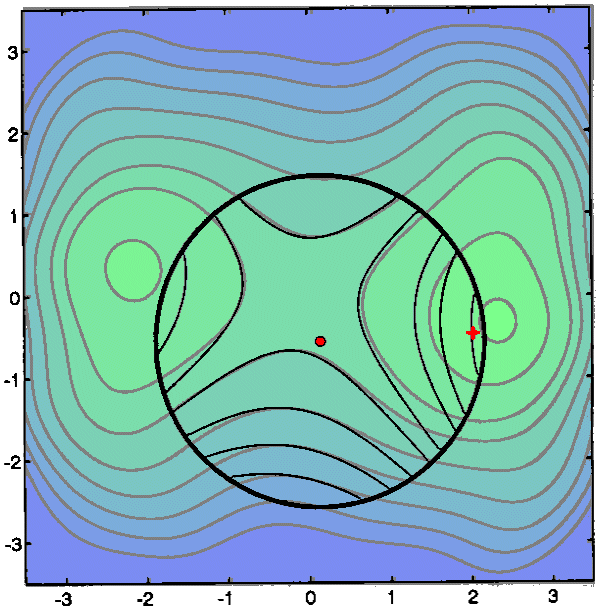
\includegraphics[width=.5\textwidth]{trm/Image5.png}
\end{frame}
%-----------------------------------------------------
\begin{frame}[noframenumbering]
\frametitle{Illustration (source : F. Vanden Berghen)}
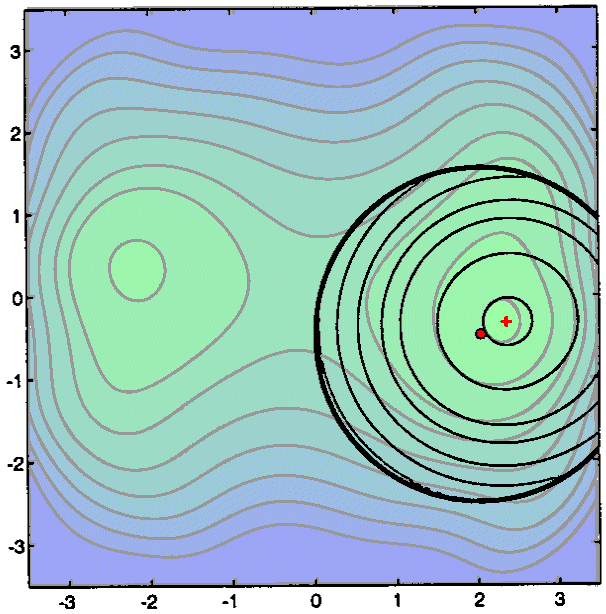
\includegraphics[width=.5\textwidth]{trm/Image6.png}
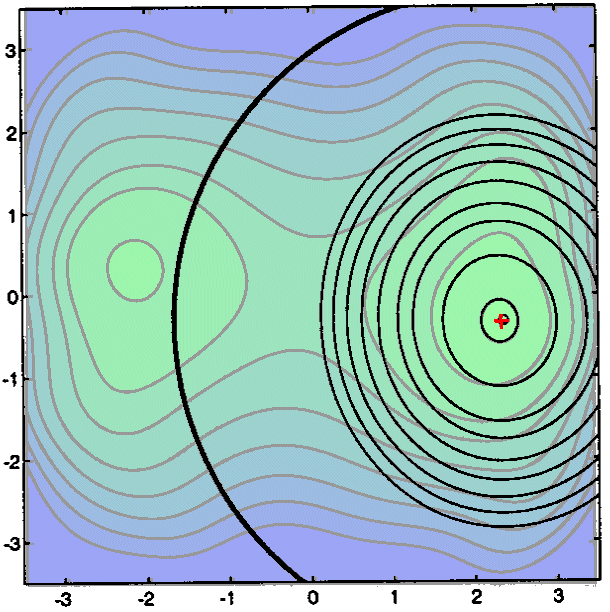
\includegraphics[width=.5\textwidth]{trm/Image7.png}
\end{frame}
%-----------------------------------------------------
\begin{frame}
\frametitle{Avantages et inconvénients}
\begin{block}{Avantages}
\begin{itemize}
 \item Garantie de convergence
 \item Méthodes assez parcimonieuses
 \item Robuste
 \item Accepte un assez grand nombre de variables
\end{itemize}
\scriptsize{
 \begin{thebibliography}{1}
\beamertemplatearticlebibitems
     \bibitem{conn}
     Conn, Scheinberg, and Vicente
         \newblock Introduction to derivative-free optimization
         \newblock MPS-SIAM Series on Optimization (2009)
 \end{thebibliography}}
\end{block}

\begin{alertblock}{Méthode locale}
\begin{itemize}
 \item Pas de métamodèle final utilisable globalement
 \item Proche des méthodes de gradient
\end{itemize}
\end{alertblock}
\end{frame}
